En esta sección se describe el diseño completo del Front-End analógico compatible con la norma ISO/IEC 14443A. En la próxima sección se verán los resultados y mediciones del diseño. 

\subsection{Diseño de un CI}
El diseño de circuitos integrados se mantiene
siempre dentro de cierto número de pasos que
no varían con el circuito. Estos pasos pueden
detallarse en los ítems que se muestran a continuación \cite{detect_fallas_500nm}.

\begin{enumerate}
\item Diseño teórico: definición del comportamiento
deseado y elección de la topología del circuito.
\item Descripción del comportamiento: iteración de
simulaciones y modificaciones hasta la obtención
del comportamiento deseado.
\item Layout: realización, en el software especializado
(Synopsys Custom Designer en nuestro
desarrollo), del diseño físico en silicio del
circuito, a partir de las reglas de diseño de la
tecnología.
\item Design Rules Check (DRC), Layout vs. Schematic
(LVS) y Parasitic Extraction (PEX): análisis
correspondientes a la verificación del diseño.
En esta etapa se realiza la búsqueda, en
el layout, de violaciones a las reglas de diseño
(DRC). Luego, se verifica que el layout y el esquemático
diseñados correspondan el uno con
el otro (LVS). Al final, se realiza una simulación
teniendo en cuenta los componentes parásitos
que aparecen en el diseño físico (PEX). Las herramientas
utilizadas para esto son Mentor Graphics y Synopsys.
\item Iteración en el diseño: si en el transcurrir de
alguno de los pasos no se cumple con el comportamiento
estipulado del diseño, se retorna al
ítem número 2 y se vuelven a realizar los pasos
posteriores hasta encontrar el comportamiento
deseado y detallado en el ítem 1.
\end{enumerate}

\subsection{Descripción general de funcionamiento}

\begin{figure}[H]
\centering
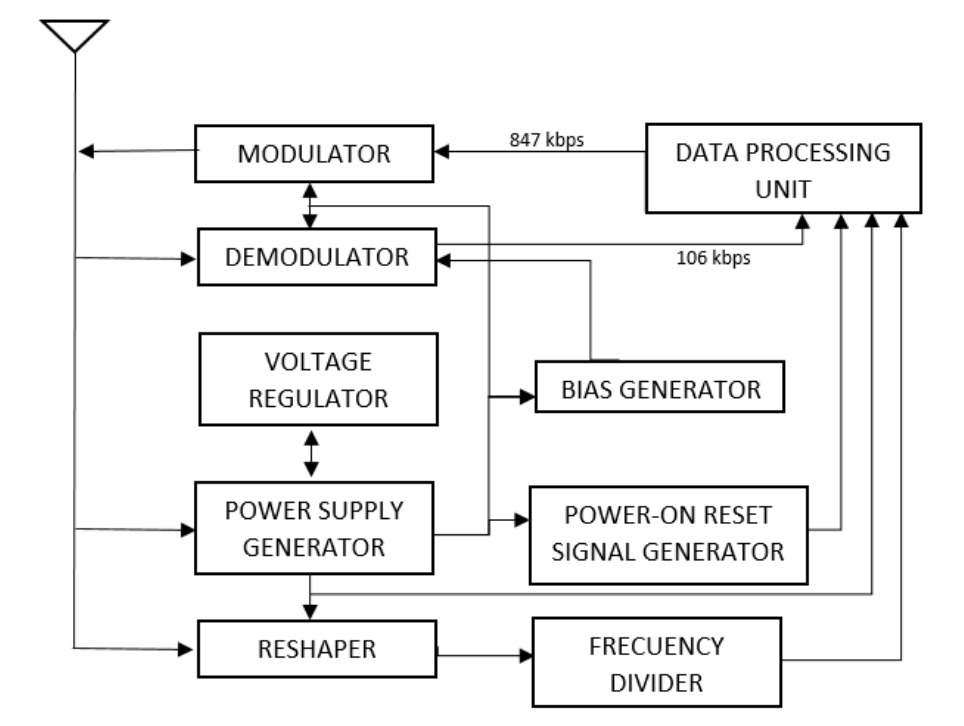
\includegraphics[scale=0.4]{modulos_rfid.png}
\caption{Módulos Front-End Analógico}
\label{fig:modulos_rfid}
\end{figure}

La tarjeta de contacto consiste en dos secciones principales: Sección de RF (Front-End Analógico) y la Unidad de Procesamiento de Datos (DPU). Los módulos del Front-End Analógico (AFE) se muestra en la figura \ref{fig:modulos_rfid}, el cuál consiste en un generador de tensión \textit{(Power Supply Generator - PSG)}, un generador de clock \textit{(Clock Generator - CG)}, un regulador de tensión continua \textit{(Voltage Regulator - VR)}, un \textit{Power On Reset (POR)}, un modulador y un demodulador.

El principio de funcionamiento es lo siguiente: 

\begin{itemize}
\item Cuando el PICC (tag) entra a un campo electromagnético, osea, cuando se acerca al PCD (lector), induce una tensión en la antena del PICC y energiza el módulo PSG. 
\item PSG contiene un rectificador de tensión alterna y un regulador Shunt (Figura \ref{fig:modulos_picc}). Éste módulo tiene como propósito entregar una tensión continua a la salida y limitar la tensión máxima de operación que puede soportar el chip. La salida limitada en tensión va conectado a la entrada de VG. 
\item VG regula la entrada y provee una tensión constante a la salida de la misma. Éste módulo es muy importante ya que alimenta a todo el chip. 
\item El POR entrega un cero lógico por un tiempo determinado al recibir la alimentación de VG. Ésto sirve para resetear todos los flip flops de la DPU. 
\item El modulador y demodulador son módulos analógicos que sirven para que el PCD se pueda comunicar con el PICC.
\end{itemize}

\begin{figure}[H]
\centering
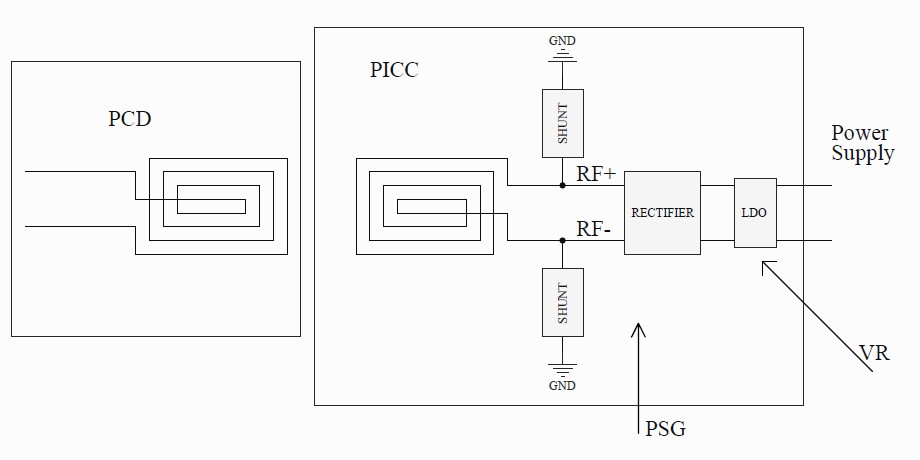
\includegraphics[scale=0.5]{picc.png}
\caption{Módulos PICC (Power Management)}
\label{fig:modulos_picc}
\end{figure}

A continuación se describe detalladamente el funcionamiento de cada módulo del AFE.


\subsection{Generador de Tensión (PSG)}

El PSG se divide en dos partes: rectificación de la fuente de alterna (13,56 MHz) y límitación de potencia. 

La primera parte cumple la función de rectificar el campo magnético inducido desde el lector. Se implementó un rectificador con transistores NMOS funcionando como diodo. En la figura \ref{fig:rectifier} se puede ver la topología implementada. 

\begin{figure}[H]
\centering
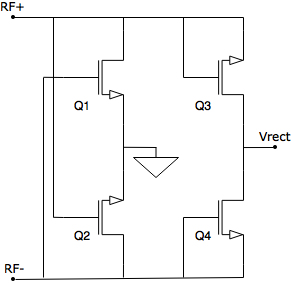
\includegraphics[scale=0.6]{circuitos/Rectifier.png}
\caption{Rectificador de onda completa con transistores NMOS}
\label{fig:rectifier}
\end{figure}

Cabe destacar que la caída de tensión sobre el rectificador depende inversamente con el ancho de canal (W) del MOS. Mientras más ancho es W, menos tensión cae en esta etapa. Es lógico que el limitante en éste caso es el área. 

La segunda parte cumple la función de proteger el chip, ya que para que el chip sea compatible con la norma ISO/IEC 14443-2, el PICC debe ser capaz de funcionar para distintas intensidades de campo magnético (1,5-7,5 A/m rms). En la figura \ref{fig:shunt} se muestra la topología.

\begin{figure}[H]
\centering
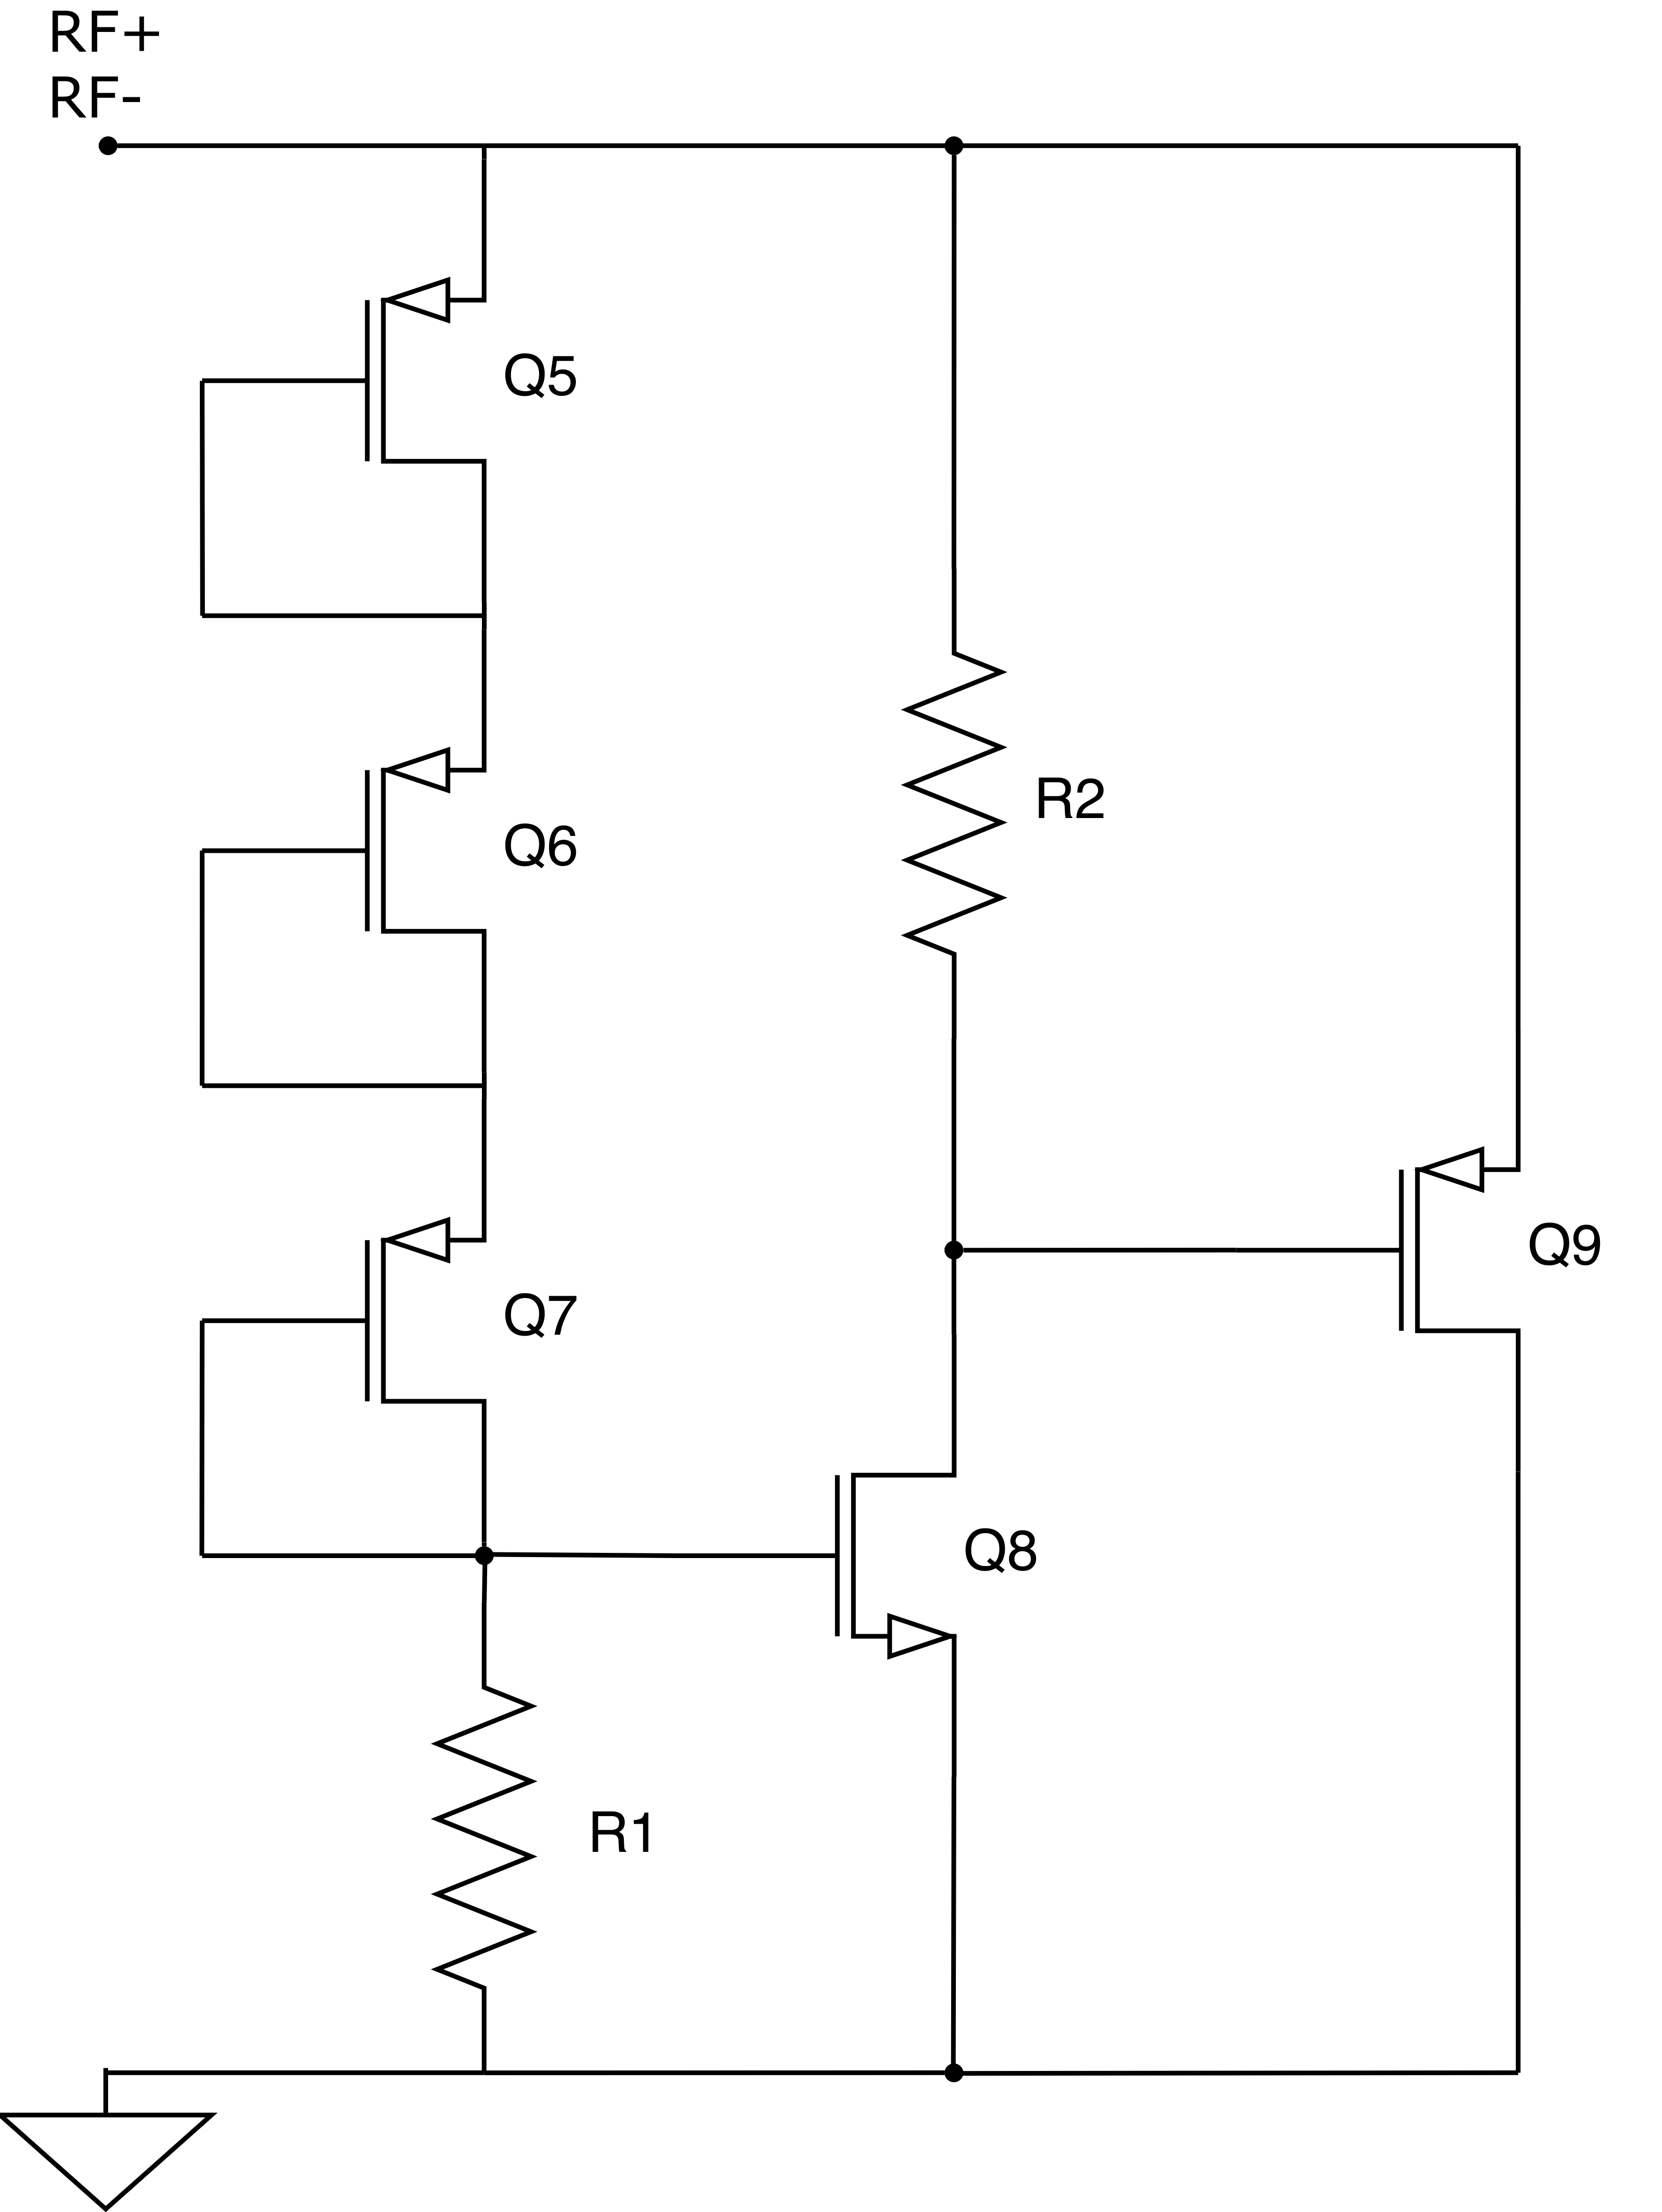
\includegraphics[scale=0.045]{circuitos/Shunt.png}
\caption{Limitador de potencia - Shunt}
\label{fig:shunt}
\end{figure}

El limitador shunt tiene como característica prender el transistor Q9 al superar una tensión de umbral en los bornes del módulo, osea que, éste transistor trabaja idealmente sólo en corte y saturación. 

Como las dos tecnologías que se utilizó tienen distintas tensiones de operación (3,3 a 5 V para ONC5 y 1,2 a 2,5 V para GF130), las tensiones de umbral varían. En las figuras \ref{fig:shunt_500} y \ref{fig:shunt_130} se muestran las tensiones de umbral para cada tecnología. Como se puede observar, para ONC5 el circuito se prende en 4,5 V y para GF130 se prende en 2,8 V.

Entre el rectificador y el shunt se encuentra un capacitor de aproximadamente 400 pF, éste capacitor depende de la tensión de operación de la tecnología y del proceso. 

\begin{figure}[H]
\centering
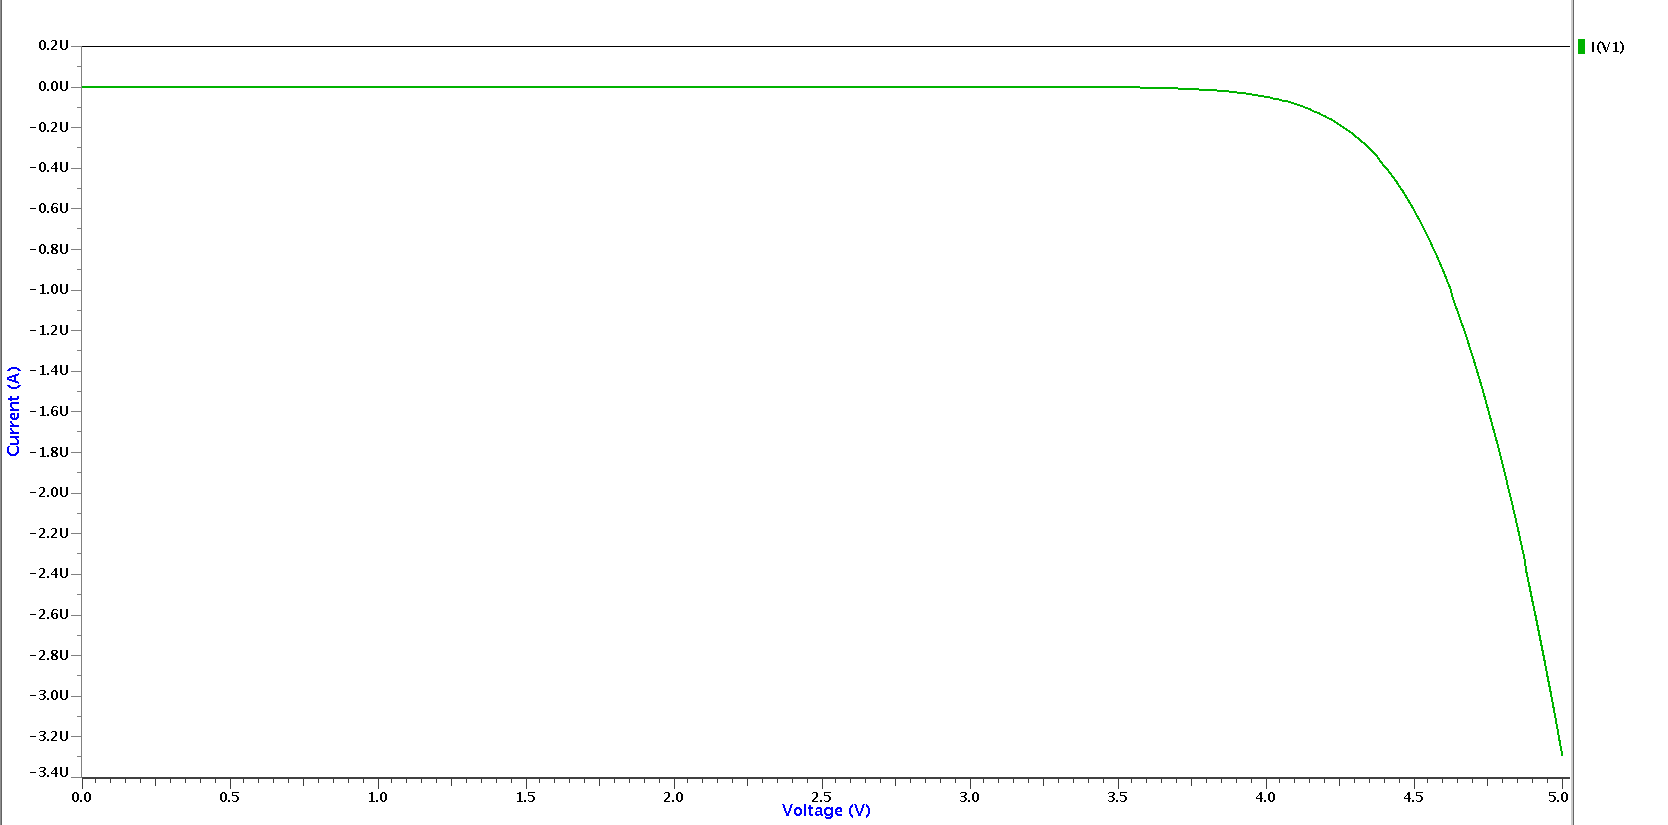
\includegraphics[width=0.9\linewidth]{simulaciones/shunt_500.png}
\caption{Tension de umbral (ONC5)}
\label{fig:shunt_500}
\end{figure}

\begin{figure}[H]
\centering
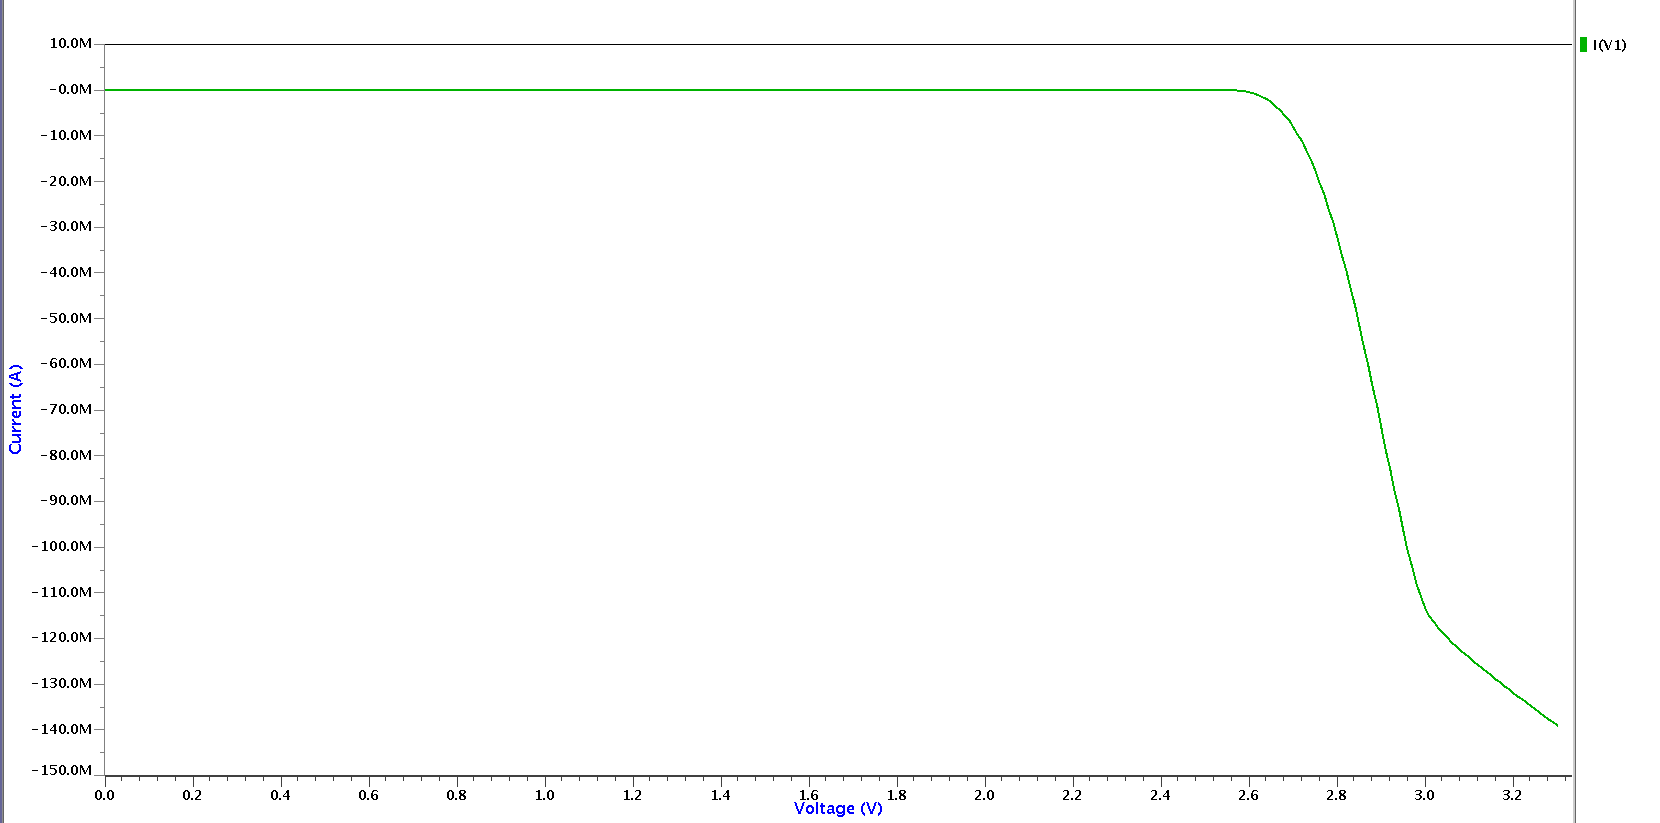
\includegraphics[width=0.9\linewidth]{simulaciones/shunt_130.png}
\caption{Tension de umbral (GF130)}
\label{fig:shunt_130}
\end{figure}


\subsection{Generador de clock (CG)}

El generador de clock obtiene el reloj a partir de la antena, ya que el lector emite una frecuencia de 13,56 MHz +- 7 kHz, que está especificado en la norma ISO/IEC 14443-2 \ref{sec:iso}. El módulo (figura \ref{fig:clock_gen}) consiste principalmente en dos Flip Flop tipo D (que actúa como divisor de clock por 2) y una compuerta XOR.

Básicamente funciona de la siguiente manera: Aprovechando la diferencia de fase entre los bornes de la antena con respecto a masa (180 grados de diferencia de fase), se le hace pasar por los flip flop D y la XOR para recuperar el clock (figura \ref{fig:clock_gen_sim}).

\begin{figure}[H]
\centering
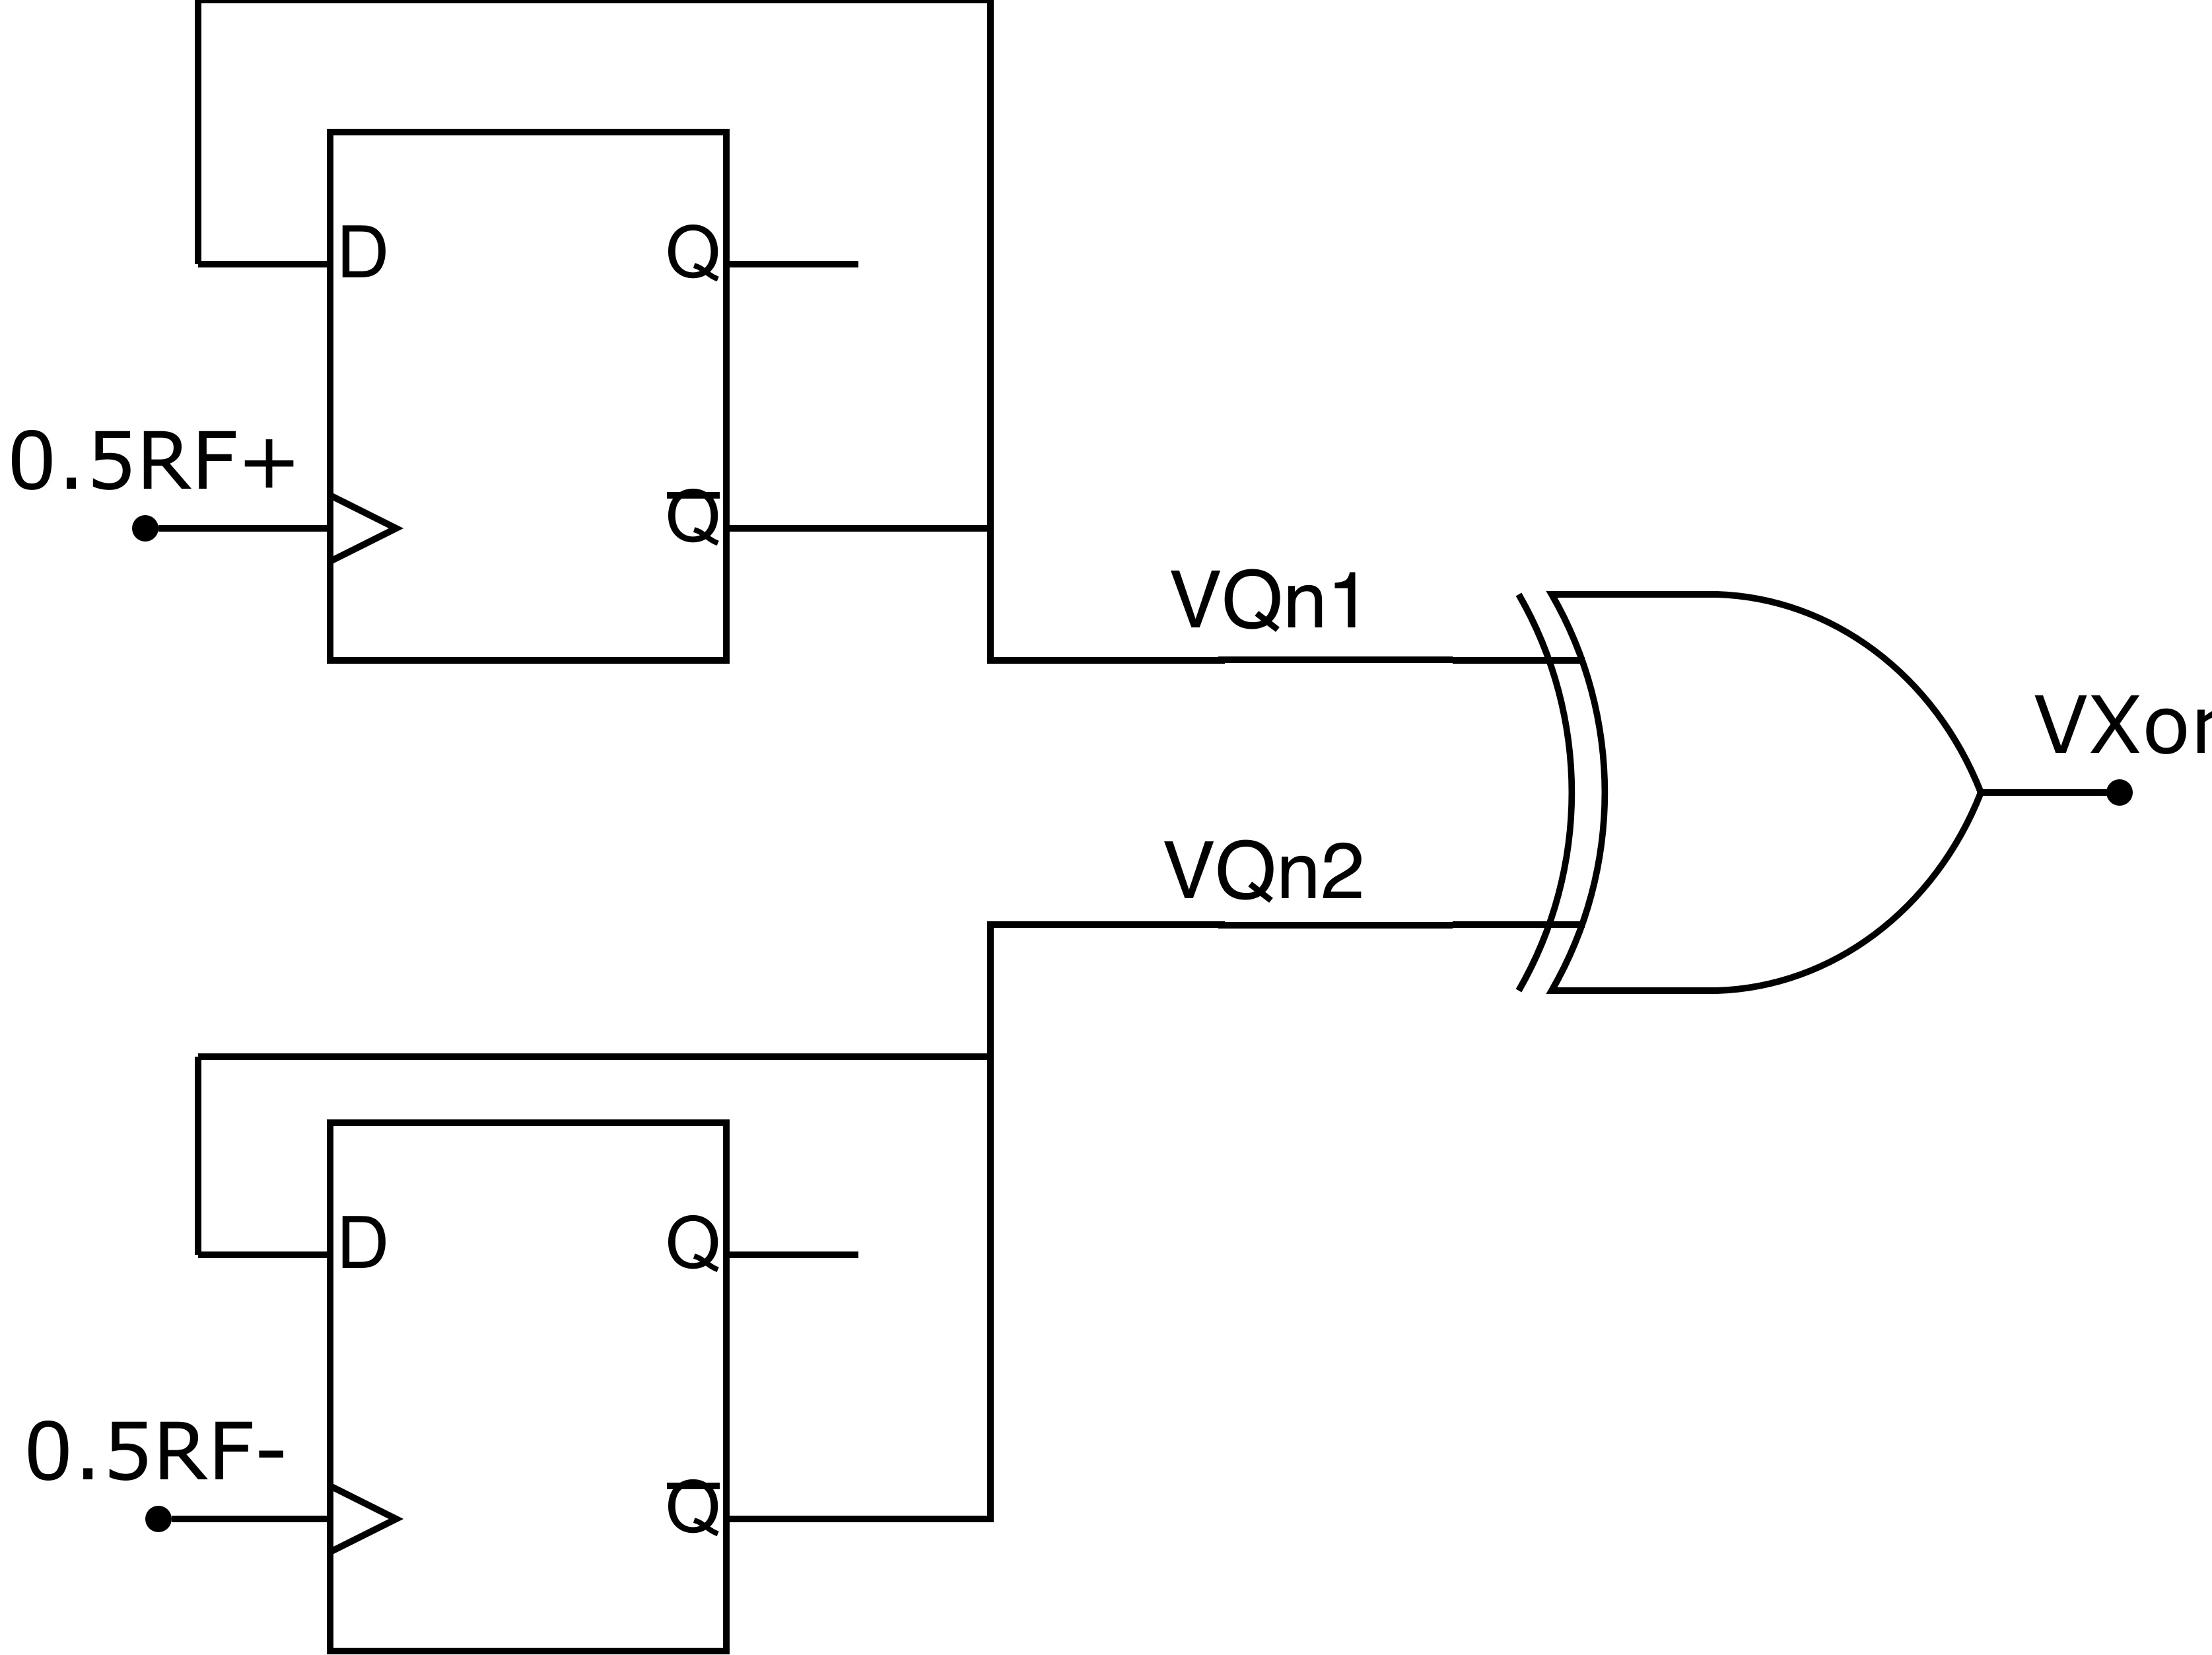
\includegraphics[width=0.5\linewidth]{circuitos/CLK.png}
\caption{Generador de clock}
\label{fig:clock_gen}
\end{figure}

\begin{figure}[H]
\centering
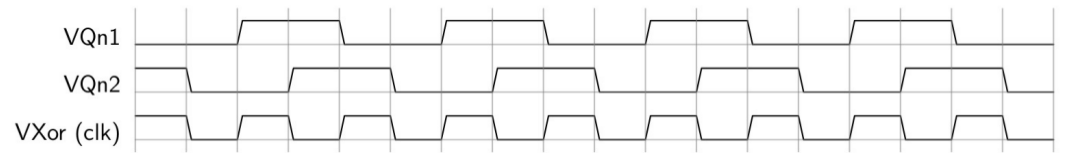
\includegraphics[width=0.9\linewidth]{circuitos/clk_sim.png}
\caption{Generador de clock (Simulación)}
\label{fig:clock_gen_sim}
\end{figure}

\subsection{Regulador de Voltaje (VR)}

El regulador de voltaje regula la tensión proveniente del PSG y provee una tensión continua constante a la salida del módulo. Éste módulo funciona como alimentación para los demás módulos del chip. La topología de la VR se puede ver en la figura \ref{fig:ldo}. Éste módulo consiste principalmente en 3 partes: Un amplificador operacional (OP-AMP) que es usado como amplificador de error (Actúa como regulación, amplifica la diferencia entre una tensión de referencia conocida con respecto a la tensión de salida); un transistor serie a la salida que es usado como amplificador de corriente; R3 y R4 son usados como divisor de voltaje resistivo (Ecuación \ref{eq:vref}).  

\begin{figure}[H]
\centering
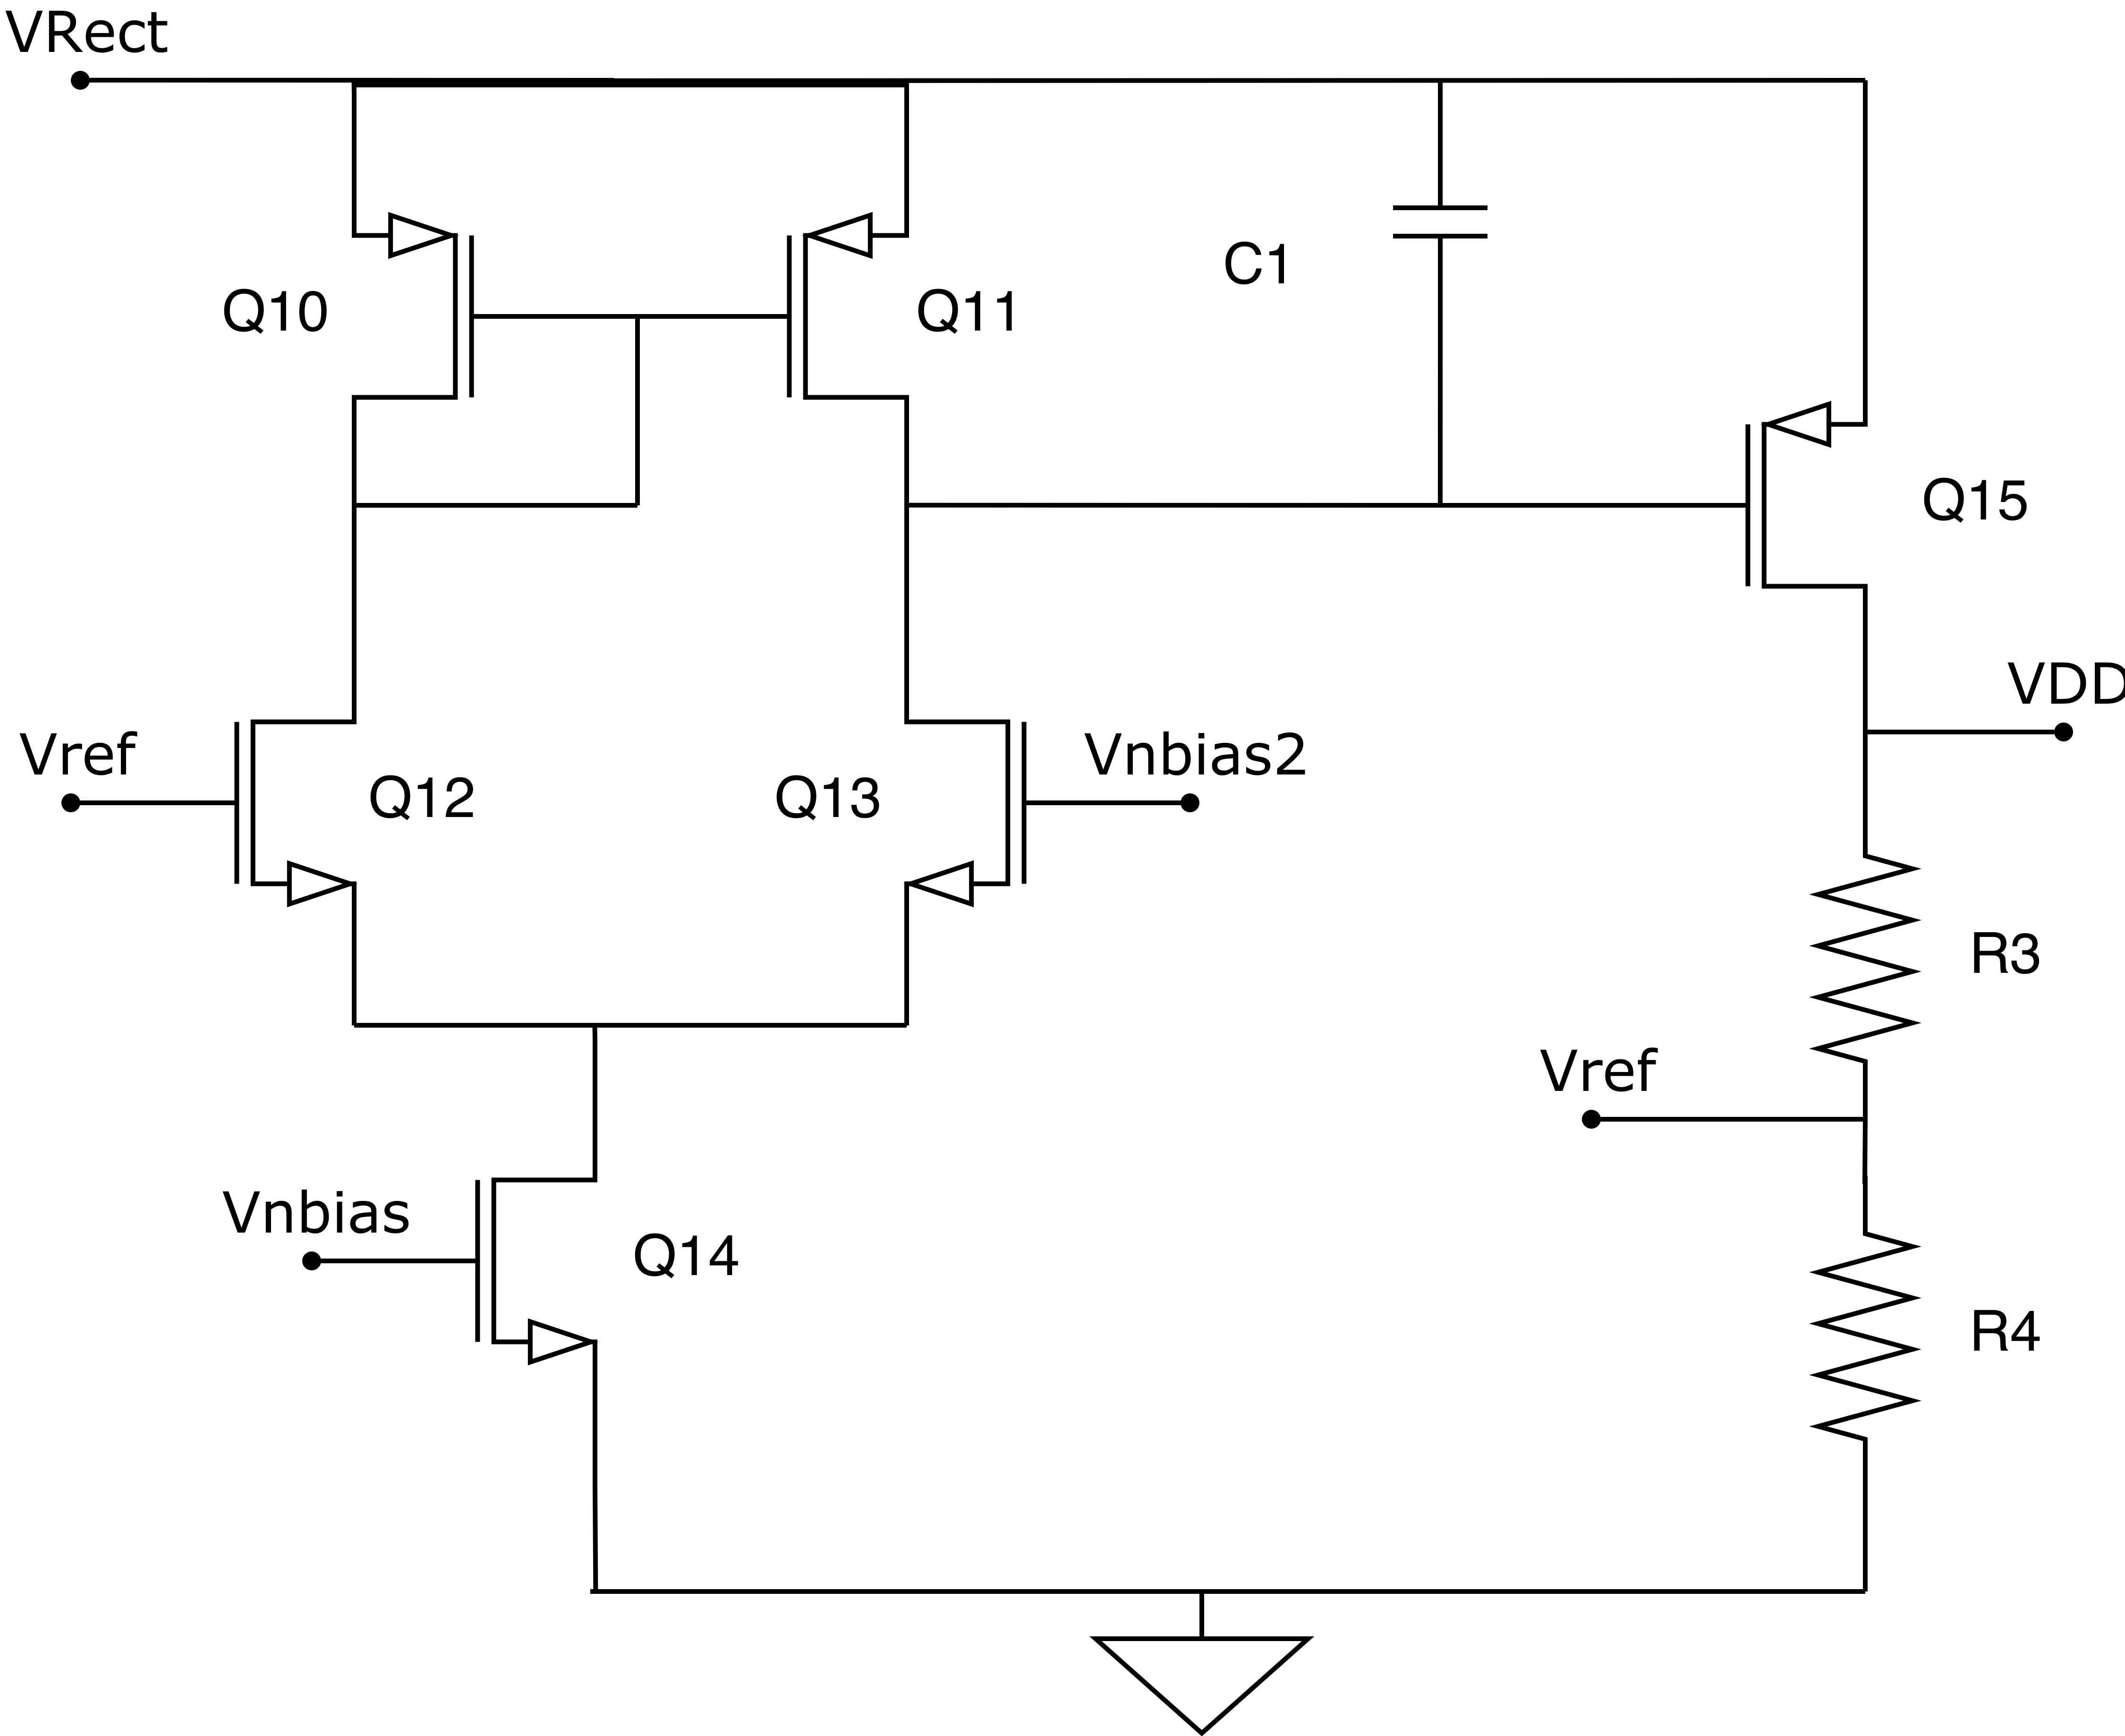
\includegraphics[width=0.5\linewidth]{circuitos/LDO.png}
\caption{Regulador de Voltage}
\label{fig:ldo}
\end{figure}

\begin{equation} \label{eq:vref}
VDD = Vref*(1+R3/R4)
\end{equation}

\subsection{Modulador}

El modulador cambia la impedancia que vista desde la PCD. Existen dos tipos de modulación: modulación resistiva y capacitiva. Ambos tipos crean una subportadora cerca de 13.56MHz. Se adoptó la modulación resistiva para éste diseño. La topología se muestra en la figura \ref{fig:mod}. Para más información, ver la sección \ref{subsec:modulador}.

\begin{figure}[H]
\centering
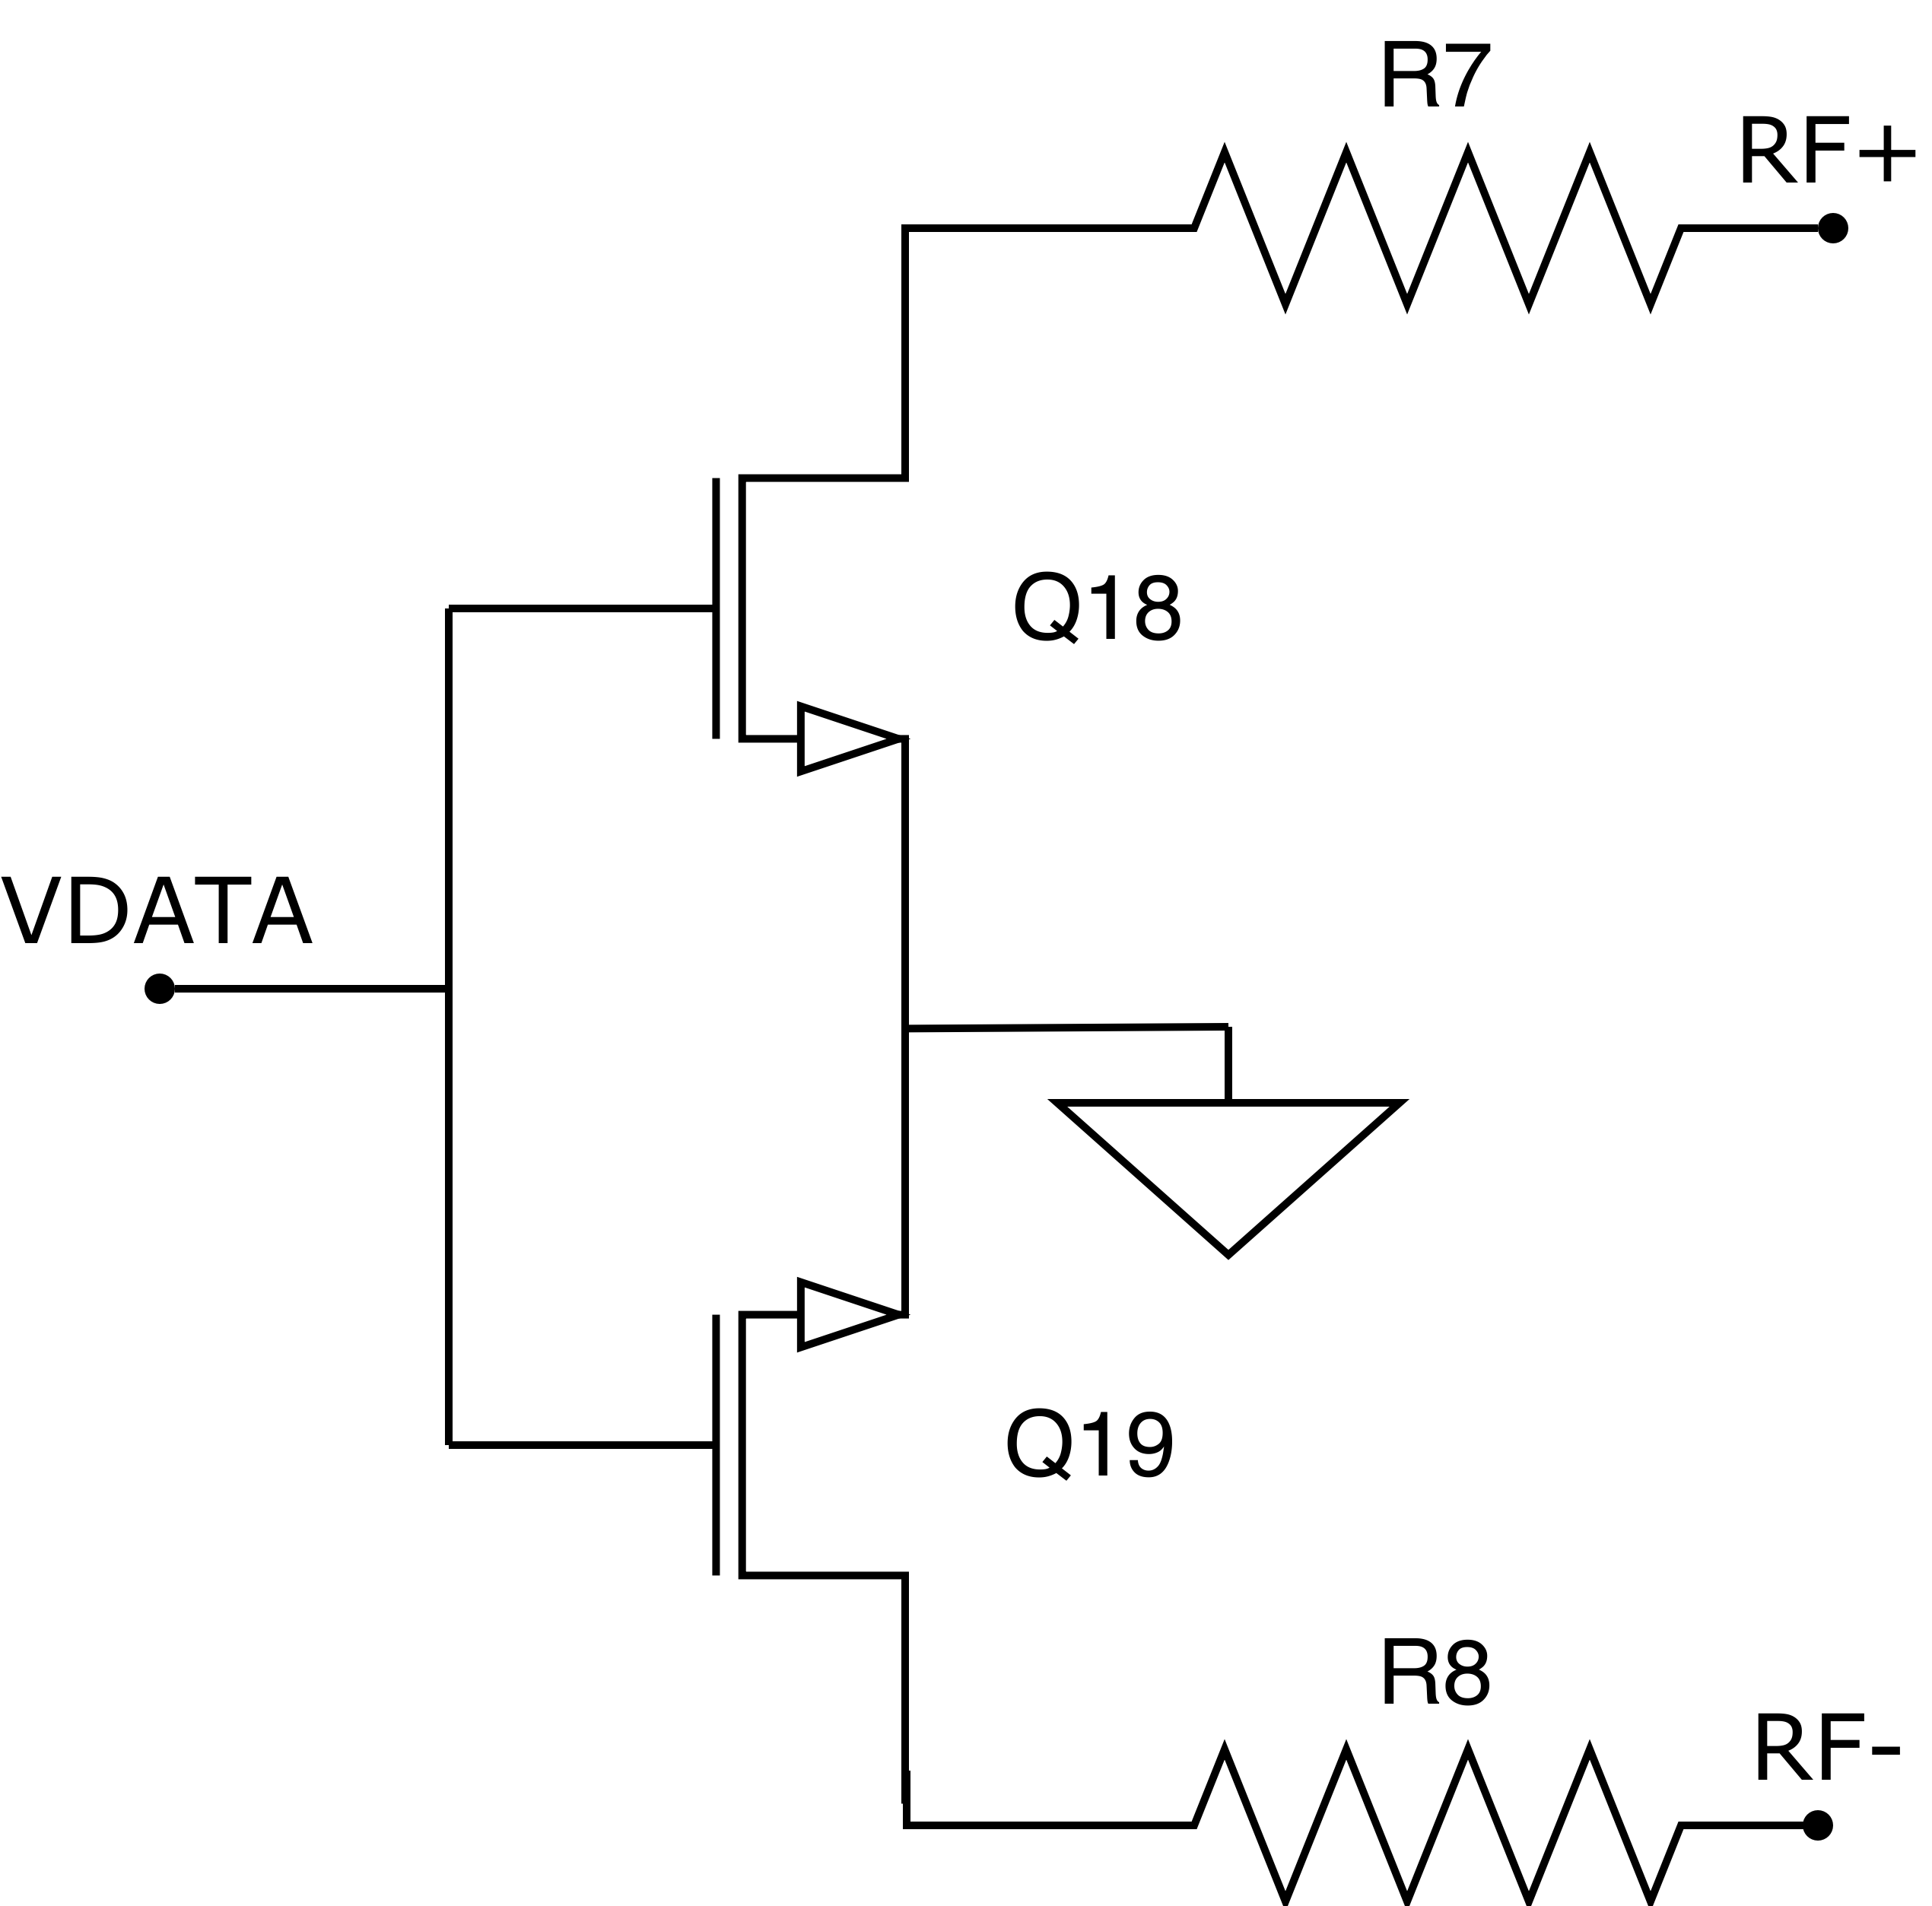
\includegraphics[width=0.3\linewidth]{circuitos/MOD.png}
\caption{Modulador}
\label{fig:mod}
\end{figure}

\subsection{Demodulador}

El demodulador recupera la trama digital transmitido por el PCD. Para el tag tipo A, se extraen los datos con un detector de envolvente. La salida del detector de envolve se conecta a un buffer. La topología se muestra en la figura \ref{fig:demod}. Para más información, ver sección \ref{subsec:demodulador}.

\begin{figure}[H]
\centering
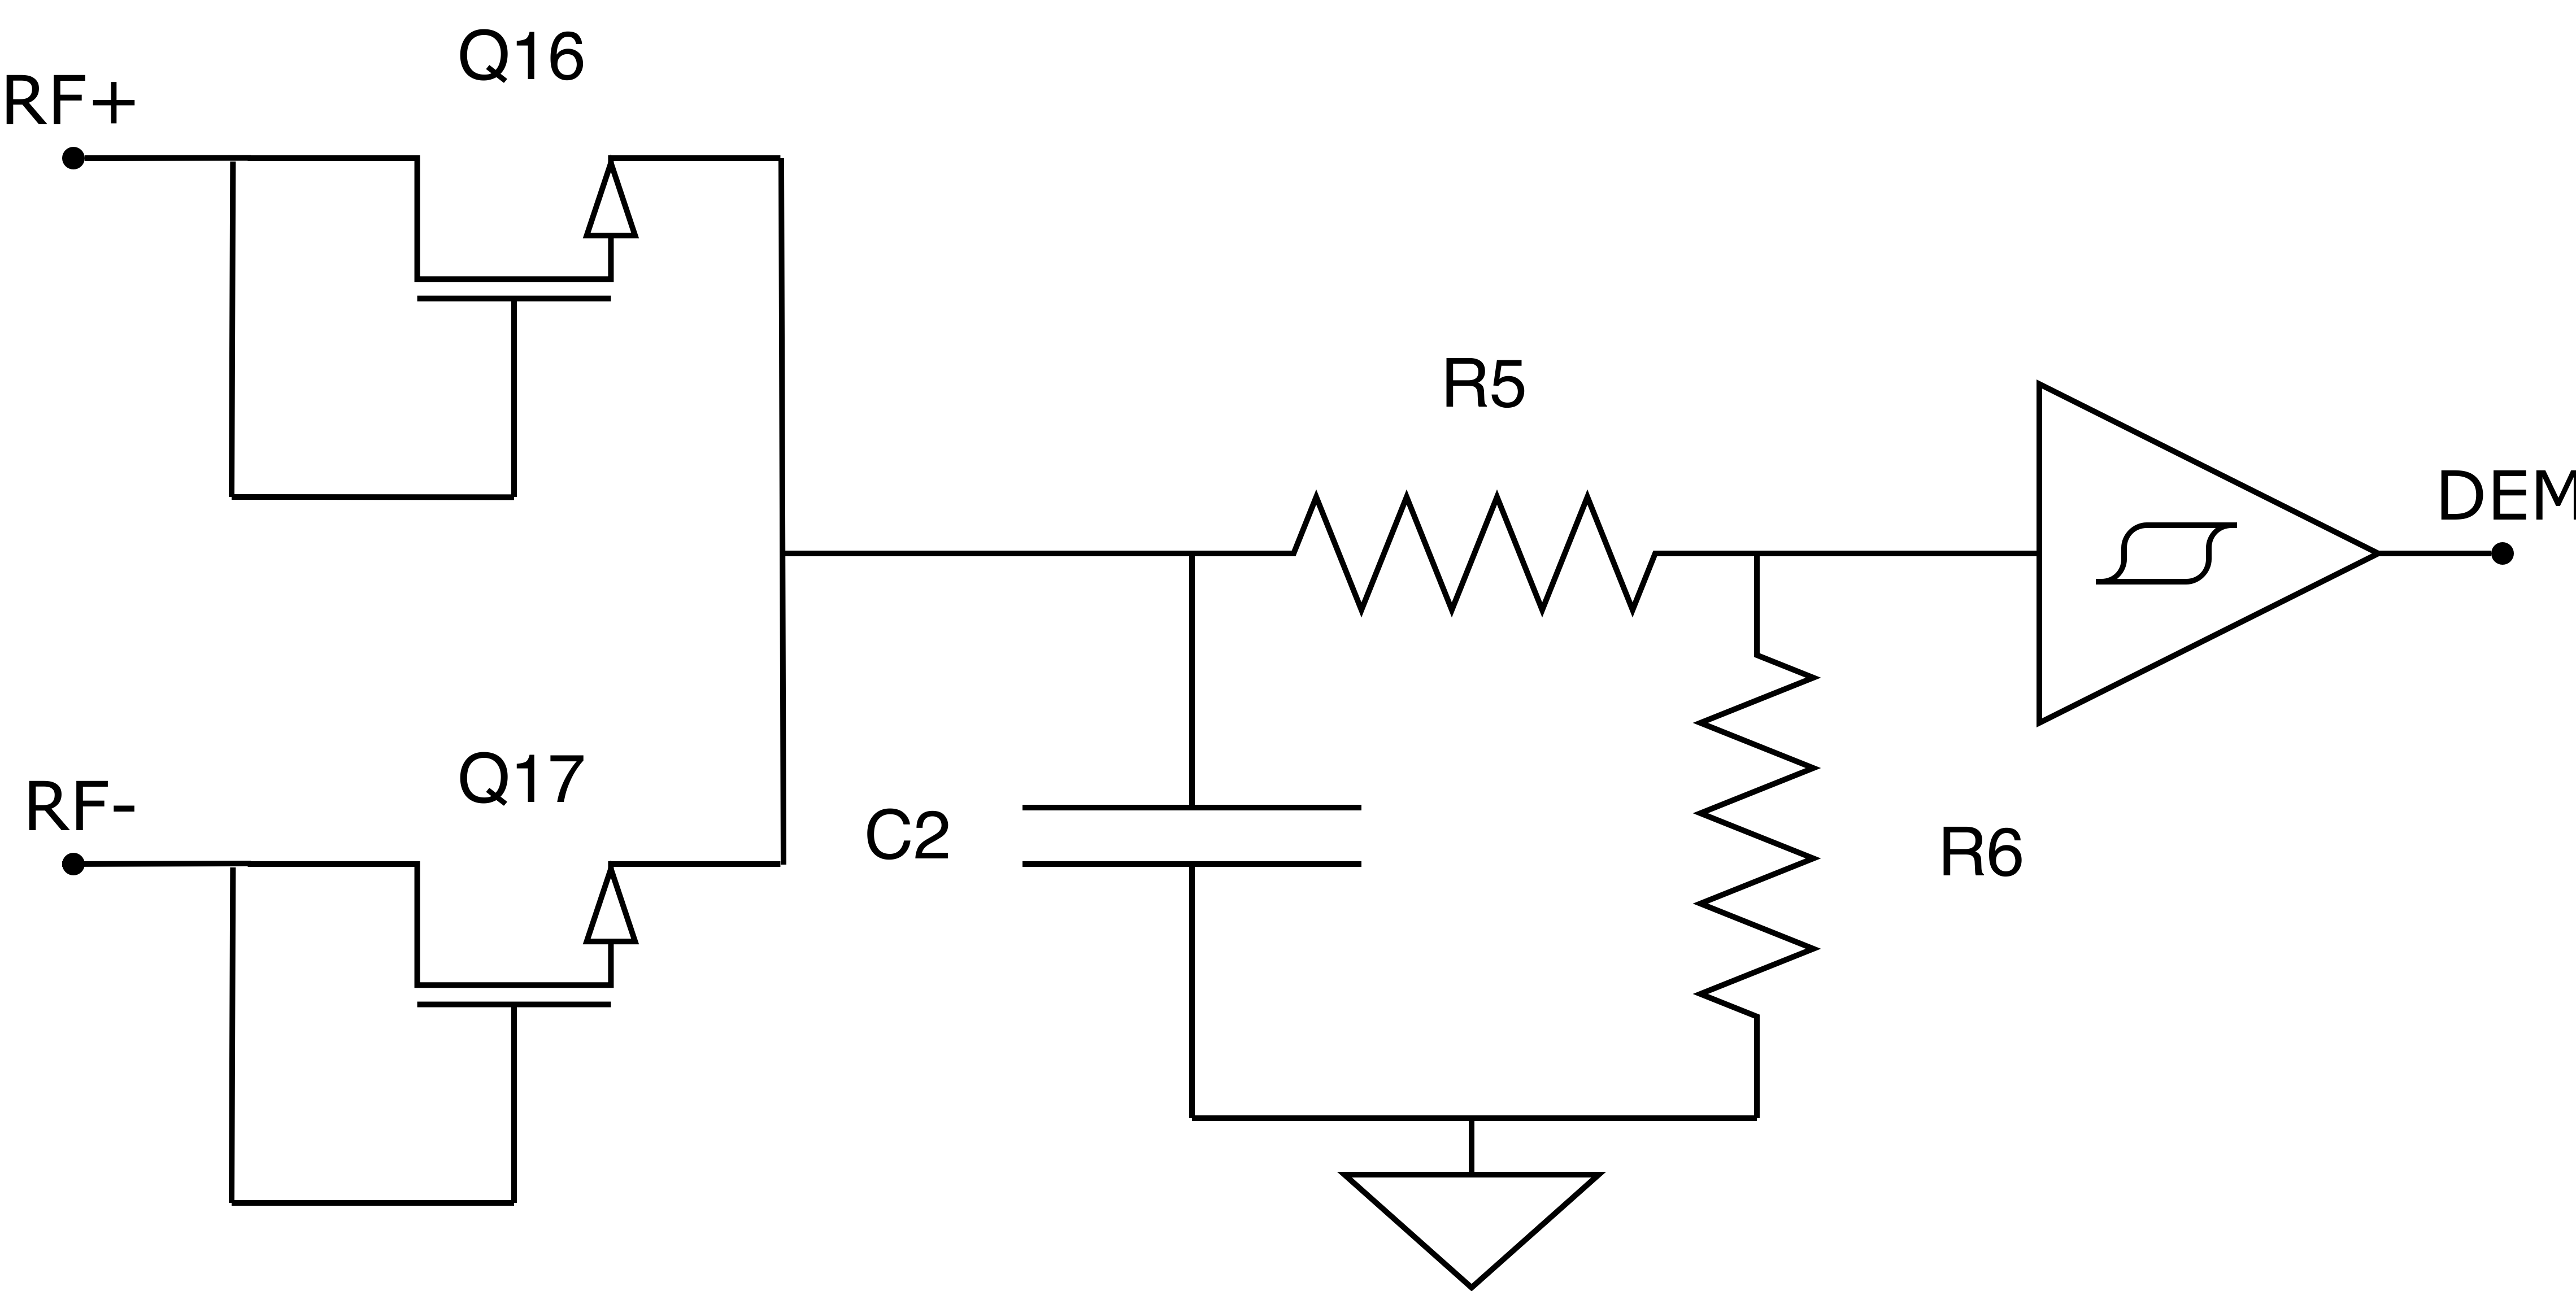
\includegraphics[width=0.7\linewidth]{circuitos/DEM.png}
\caption{Demodulador}
\label{fig:demod}
\end{figure}

\subsection{Power On Reset (POR)}

Éste módulo es usado para resetear la máquina digital (\textit{NFC Digital Core}) cuando se acerca la PICC a la PCD. La POR consiste principalmente en un filtro pasabajos RC y un buffer. El esquemático se muestra en la figura \ref{fig:por}.

\begin{figure}[H]
\caption{Power on Reset}
\label{fig:por}
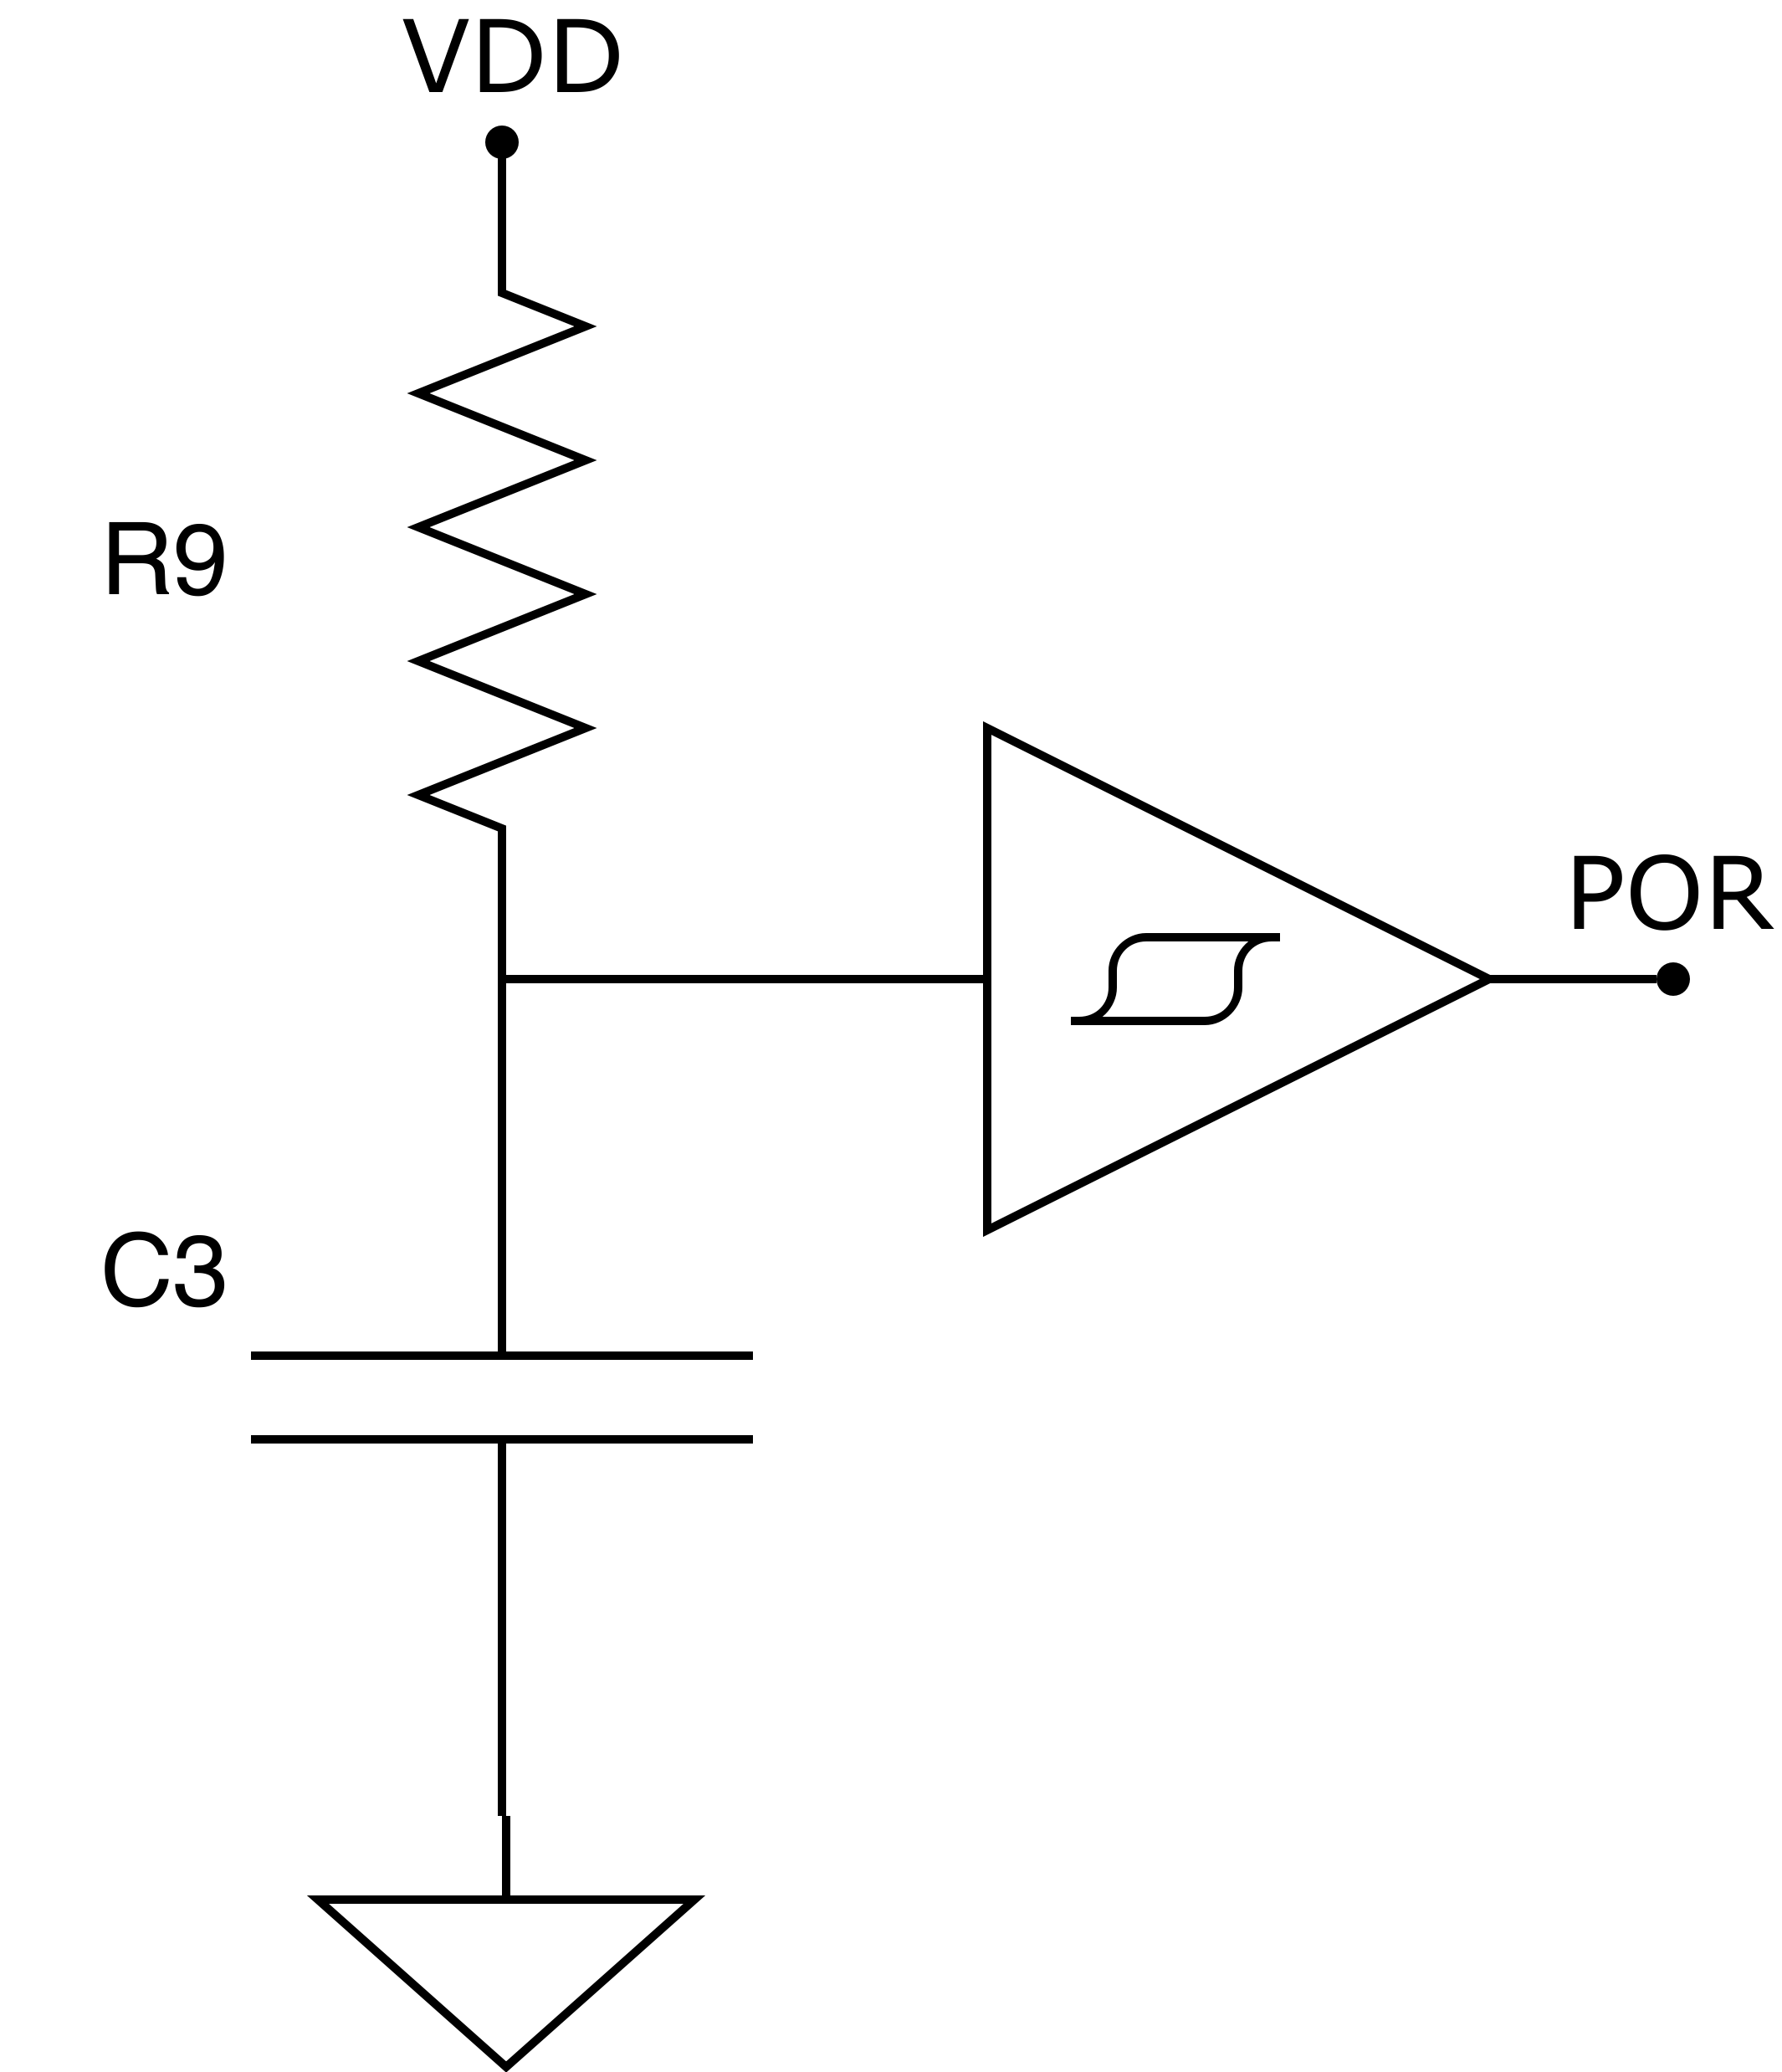
\includegraphics[width=0.3\linewidth]{circuitos/POR.png}
\centering
\end{figure}

\subsection{Diseño final}

Los valores de los componentes que se utilizó para el diseño y fabricación del proceso GF130 se puede ver en las tablas \ref{table:trans_specs_130} y \ref{table:res_specs_130}. Y los valores para el proceso ONC5 se encuentran en las tablas \ref{table:trans_specs_500} y \ref{table:res_specs_500}.


\begin{table}[H]
\centering
\begin{tabular}{c|c|c|c|c}
\textbf{Tipo}  		 & \textbf{Simbolo}	& \textbf{W}  & \textbf{L}  & \textbf{Fingers/Multiplicidad}  \\ \hline
NMOS                 & Q1,Q2,Q3,Q4    	& 10 um       & 0.4 um      & 20                \\
PMOS                 & Q5,Q6,Q7       	& 5 um        & 0.4 um      & 1                 \\
NMOS                 & Q8             	& 5 um        & 0.4 um      & 2                 \\
PMOS                 & Q9             	& 15 um       & 0.4 um      & 25                \\
PMOS                 & Q10,Q11        	& 1 um        & 3 um        & 2                 \\
NMOS                 & Q12,Q13        	& 2 um        & 1 um        & 2                 \\
NMOS                 & Q14            	& 0.5 um      & 3 um        & 1                 \\
PMOS                 & Q15            	& 10 um       & 0.4 um      & 10                \\
NMOS                 & Q16,Q17        	& 5 um        & 0.4 um      & 1                 \\
NMOS                 & Q18,Q19        	& 3 um        & 0.4 um      & 10                \\
\end{tabular}
\caption{Transistores GF130}
\label{table:trans_specs_130}
\end{table}

\begin{table}[H]
\centering
\begin{tabular}{c|c}
\textbf{Simbolos} 	&	\textbf{Valores} \\ \hline
R1              	& 10 k           \\
R2              	& 48.5 k         \\
R3,R4           	& 343 k          \\
R5,R6           	& 37.5 k         \\
R7,R8           	& 370            \\
R9              	& 150 k           \\
C1              	& 5p             \\
C2              	& 3.5 p          \\
C3              	& 7.8 p          \\
\end{tabular}
\caption{Componentes Adicionales GF130}
\label{table:res_specs_130}
\end{table}

\begin{table}[H]
\centering
\begin{tabular}{c|c|c|c|c}
\textbf{Tipo}  		 & \textbf{Simbolo}	& \textbf{W}  & \textbf{L}  & \textbf{Fingers/Multiplicidad}  \\ \hline
NMOS                 & Q1,Q2,Q3,Q4    	& 10 um       & 0.6 um      & 10                \\
PMOS                 & Q5,Q6,Q7,Q7bis   & 5 um        & 0.6 um      & 5                 \\
NMOS                 & Q8             	& 5 um        & 0.6 um      & 5                 \\
PMOS                 & Q9             	& 10 um       & 0.6 um      & 15                \\
PMOS                 & Q10,Q11        	& 12 um       & 3 um        & 1                 \\
NMOS                 & Q12,Q13        	& 3 um        & 3 um        & 1                 \\
NMOS                 & Q14            	& 1 um        & 3 um        & 1                 \\
PMOS                 & Q15            	& 10 um       & 0.6 um      & 20                \\
NMOS                 & Q16,Q17        	& 5 um        & 0.6 um      & 4                 \\
NMOS                 & Q18,Q19        	& 15 um       & 0.6 um      & 10                \\
\end{tabular}
\caption{Transistores ONC5}
\label{table:trans_specs_500}
\end{table}

\begin{table}[H]
\centering
\begin{tabular}{c|c}
\textbf{Simbolos} 	&	\textbf{Valores} \\ \hline
R1              	& 50 k           \\
R2              	& 20 k           \\
R3           	    & 280 k          \\
R4           	    & 210 k          \\
R5,R6           	& 0, 6 k         \\
R7,R8           	& 136.5          \\
R9              	& 583 k          \\
C1              	& 3.48 p         \\
C2              	& 0.336 p        \\
C3              	& 1.44 p        \\

\end{tabular}
\caption{Componentes Adicionales ONC5}
\label{table:res_specs_500}
\end{table}

El layout final del Front-end analógico (AFE) se muestran en las Figuras \ref{fig:onc5} y \ref{fig:gf130}. Fueron diseñados para los procesos On Semiconductor 500 nm (ONC5) y Global Foundries 130 nm (GF130) mencionados anteriormente. 

Para el proceso ONC5, el AFE ocupa un área de 0,7 x 0,4 mm; Mientras que para el proceso GF130, solamente 0,3 x 0,2 mm. 

\begin{figure}[H]

\subfloat[Proceso ONC5]{\label{fig:onc5}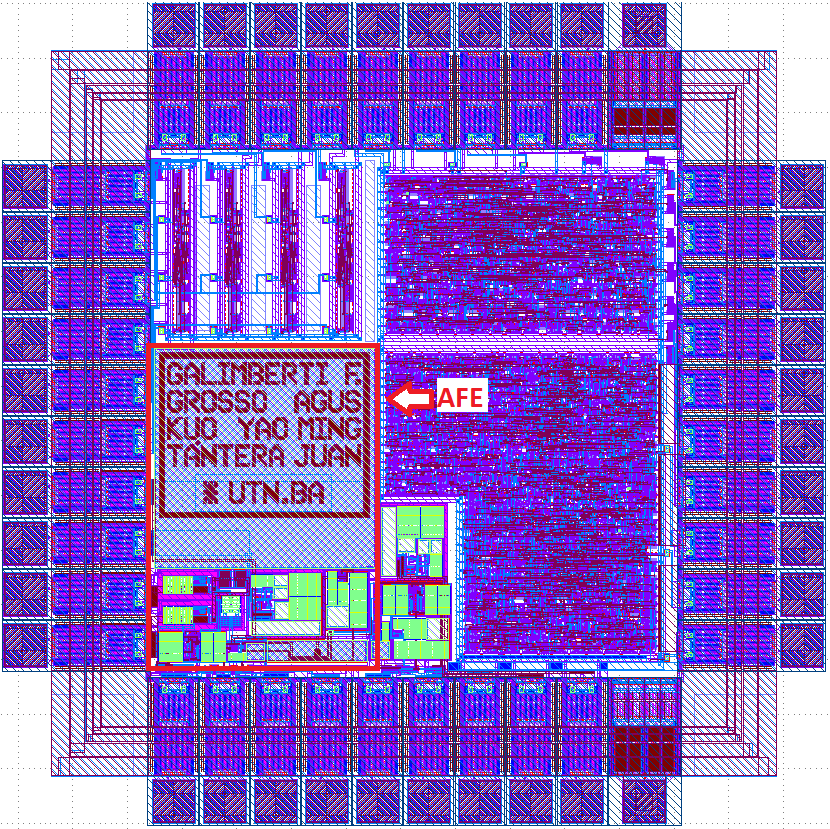
\includegraphics[width=0.5\linewidth]{circuitos/onc5_layout.png}}
\subfloat[Proceso GF130]{\label{fig:gf130}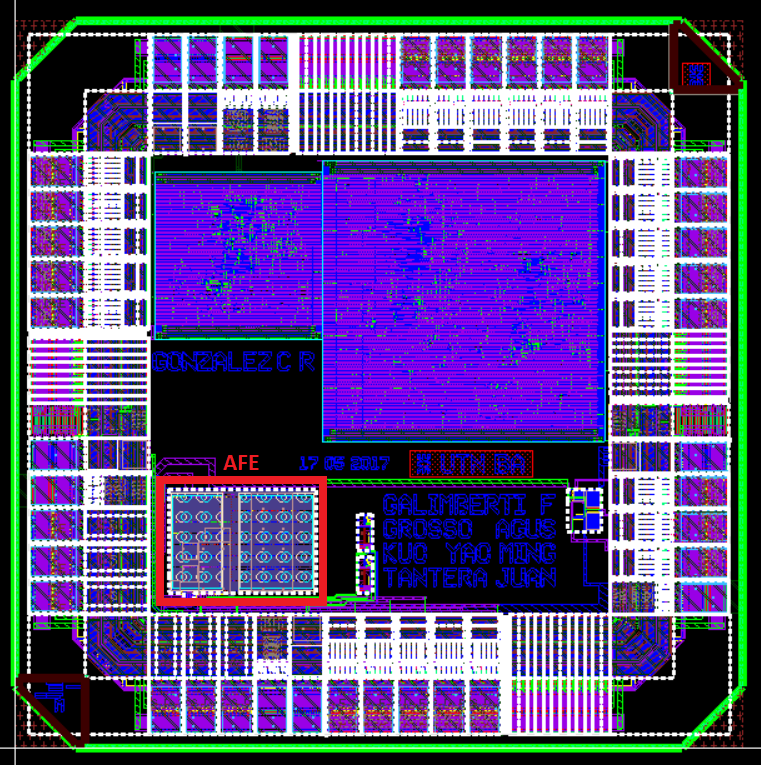
\includegraphics[width=0.5\linewidth]{circuitos/gf130_layout.png}}

\caption{Layout del Front-End Analógico}
\label{fig:layout_completo}
\end{figure}


